\documentclass[border=1pt]{standalone}
\usepackage{xfrac}%package for slanted fraction better fit into one line

\usepackage{color}
\pagecolor{white}

\usepackage{tikz}

%Some nicer color definitions
\definecolor{crimsonred}{RGB}{153,0,0}		% Neurtal red, good for dark or light bg
\definecolor{darkcharcoal}{RGB}{25,25,25}		% Darker gray
\definecolor{charcoal}{RGB}{51,51,51}		% Darker gray
\definecolor{ash}{RGB}{100,100,100}			% medium gray
\definecolor{paleblue}{RGB}{0,102,102}		% More of an `ocean' color
\definecolor{turtlegreen}{RGB}{51,153,0}	% A more neutral green
\definecolor{paleale}{RGB}{204,204,102}		% Only for dark BG
\definecolor{lager}{RGB}{140,110,10}		% Use instead of pale ale for white BG
\definecolor{regal}{RGB}{90,0,120}			% A more neutral purple
\definecolor{jeans}{RGB}{20,30,150}			% A more neutral blue
\definecolor{Alert}{RGB}{51,153,0}	


\begin{document}

	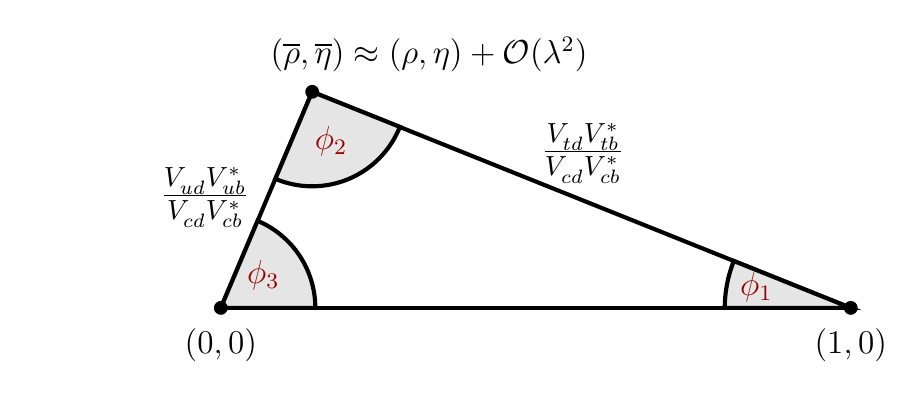
\begin{tikzpicture}[line width=1.5 pt, scale=0.8]
		\tikzstyle{every node}=[font=\large]
		\draw[]  (0,0) -- (10,0) ;
		\draw[]  (0,0) -- (1.45,3.43) ;
		\draw[]  (1.45,3.43) -- (10,0) ;
		\draw[fill=gray!20] (0,0) -- (1.5,0) arc (0:67.1:1.5) -- cycle;		
		\draw[fill=gray!20](10,0) --  (8,0) arc (180:158.15:2) -- cycle;		
		\draw[fill=gray!20] (1.45,3.43) -- (0.865933,2.04838) arc (247.1:338.2:1.5) -- cycle;	
		\node at (0.675, 0.525) {\textcolor{crimsonred}{$\phi_{3}$}};	
		\node at (8.5, 0.325) {\textcolor{crimsonred}{$\phi_{1}$}};	
		\node at (1.75, 2.65) {\textcolor{crimsonred}{$\phi_{2}$}};
		\draw (1.45,3.43) node[circle,inner sep=0pt,minimum size=5pt,fill=black,label=above:{$\phantom{(\rho,\eta)+\mathcal{O}(\lambda^{2})\approx}(\overline{\rho}, \overline{\eta})\approx (\rho,\eta)+\mathcal{O}(\lambda^{2})$}]{};
		\draw (0,0) node[circle,inner sep=0pt,minimum size=5pt,fill=black,label=below:{$(0,0)$}]{};
		\draw (10,0) node[circle,inner sep=0pt,minimum size=5pt,fill=black,label=below:{$(1,0)$}]{};
		\draw (5.75, 2.45) node[font=\Large]{$\frac{V^{}_{td}V_{tb}^{*}}{V^{}_{cd}V_{cb}^{*}}$};
		\draw (-0.25, 1.75) node[font=\Large]{$\frac{V^{}_{ud}V_{ub}^{*}}{V^{}_{cd}V_{cb}^{*}}$};
		
		%\node[right] (red) at (-4.5,3) {\Large \textcolor{jeans}{\sf Unitarity triangle}};	
		\node (reddot) at (1,2.5) {};
		%\path[->, color=jeans, line width=2.] (red) edge [out = 0, in = 180] (reddot);	
		
		%\node[right] (red2) at (5,3.3) {\Large \textcolor{jeans}{\sf Area $\propto A^{2}\lambda^{6}\eta(1-\sfrac{\lambda^{2}}{2}) = J$}};	
		\node (reddot2) at (3.5,1.2) {};
		%\path[->, color=jeans, line width=2.] (red2) edge [out = 300, in = 0] (reddot2);	
		
	\end{tikzpicture}


\end{document}